\documentclass{article}
\usepackage[pdftex]{graphicx}
\pdfcompresslevel=9
\pdfoutput=1

\topmargin 0in
\textheight 8in
\oddsidemargin 0in
\evensidemargin 0in
\textwidth 6.5in
\parskip 0.1in
\parindent 0in

\renewcommand{\arraystretch}{2}
\newenvironment{Matrix}[1]{\left[ \begin{array}{#1}}{\end{array} \right]}
\newcommand{\Real}{{\mbox{\rm I}\hspace*{-2pt}\mbox{\rm R}}}
\newcommand{\Code}[1]{{\tt #1}}

\begin{document}
\DeclareGraphicsExtensions{.pdf,.png}

\begin{center} \large\bf
  Directions for Running TriangleIntersection2.exe
\end{center}

\section{Introduction}

This is a Microsoft Windows application that is built on top of the
\Code{FWinApplication} and \Code{MagicFM} libraries.  The program illustrates
four intersection routines for triangles in 2D:
\begin{enumerate}
  \item  Test for intersection of stationary triangles.
  \item  Find the intersection set of stationary triangles.
  \item  Test for intersection of moving triangles during a specified time
    interval and report the first time of contact.
  \item  Find the intersection of moving triangles during a specified time
    interval and report the first time of contact and the intersection
    set at that time.
\end{enumerate}

When you run the program, a window is displayed and shows two triangles, one
drawn in red (triangle $0$) and one drawn in blue (triangle $1$).  Figure 1
shows the initial window.
%
% FIGURE 1
%
\begin{center}
  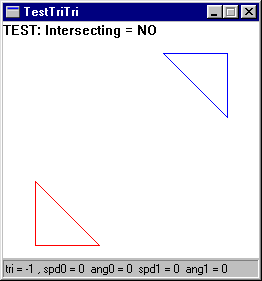
\includegraphics{Figure1.png}

  Figure 1.  The initial window for TestTriTri.exe.
\end{center}
%
The status bar shows the active triangle (initially $-1$ since no triangle is
active).  The status bar also shows the velocity of each triangle as a speed
and an angle index for an angle measured from the positive x--axis.  Given an
angle index of $N \in \{0,\ldots,31\}$, the actual angle is $\theta =
2\pi N/32$.  The initial angles are both zero, so the direction of velocity is
$(1,0)$.  The speeds are both zero, so the velocities themselves are $(0,0)$.
A triangle is activated by clicking on it with the left mouse button.  The
upper portion of the window shows the type of intersection test:  \Code{TEST},
\Code{FIND}, \Code{TEST VEL}, or \Code{FIND VEL}.  These correspond to the
four tests mentioned above, in that order.  To toggle among the types, press
the \Code{`t'} key.  After the type is a statement about whether or not the
triangles are intersecting.

\section{Moving the Triangles}

You can move a triangle by clicking on an interior point with the left mouse
button and dragging to a new location.  In the \Code{TEST} case, Figure 2
shows the two stationary triangles that have been dragged so that they
intersect.
%
% FIGURE 2
%
\begin{center}
  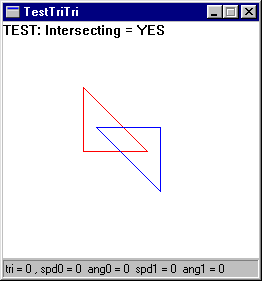
\includegraphics{Figure2.png}

  Figure 2.  Two intersecting triangles in the \Code{TEST} query.
\end{center}

\section{Changing the Triangle Vertices}

You can also change a triangle vertex by clicking with the left mouse button
near a vertex and dragging it.  Figure 3 shows the two stationary triangles
that have been modified and moved.  The \Code{FIND} case is used.  In this
case, the intersection section set is calculated and displayed in purple.
%
% FIGURE 3
%
\begin{center}
  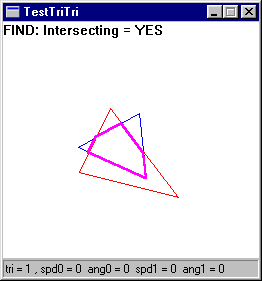
\includegraphics{Figure3.png}

  Figure 3.  Two modified and intersecting triangles in the \Code{FIND} query.
\end{center}

\section{Changing the Triangle Velocities}

Activate the triangle whose velocity you want to change.  The speed can be
modified by pressing the \Code{`<'} and \Code{`>'} keys.  The minimum speed
is zero and the maximum speed is $64$.  The angle index can be modified by
pressing the \Code{`+'} and \Code{`-'} keys.  In the \Code{TEST} and
\Code{FIND} cases, only the status bar changes.  However, in the
\Code{TEST VEL} and \Code{FIND VEL} cases, triangles are drawn in dark red
and dark blue that correspond to the original triangles moved by their
velocities over an interval of $1$ unit of time.  The paths of the vertices
over that time interval are also drawn.  Figure 4 shows a typical image for
two modified and moved triangles in the \Code{TEST VEL} case.
%
% FIGURE 4
%
\begin{center}
  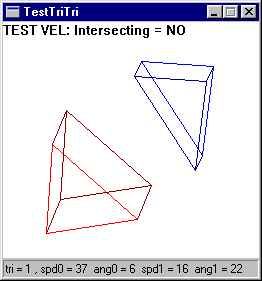
\includegraphics{Figure4.png}

  Figure 4.  Two modified and moved triangles in the \Code{TEST VEL} query,
  both triangles having nonzero velocities.
\end{center}

\section{Test or Find Intersections for Moving Triangles}

In the cases \Code{TEST VEL} and \Code{FIND VEL}, if the triangles do
intersect at first time $T \in [0,1]$, the program draws the triangles moved
only over the interval $[0,T]$ so that they are just touching.  As you drag
one original triangle towards the other, you will notice that the moved
triangles vary in distance from the originals, this being the case since $T$
is changing as you drag the triangles.  If $T = 0$, the triangles are
initially intersecting.  In the case \Code{FIND VEL}, the intersection set at
first time of contact is drawn in purple, either a single point or a line
segment.  If $T = 0$ in this case, the polygon of intersection is drawn.
Figure 5 shows a case where $T > 0$.
%
% FIGURE 5
%
\begin{center}
  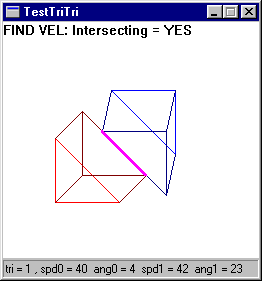
\includegraphics{Figure5.png}

  Figure 5.  Two modified and moved triangles in the \Code{FIND VEL} query,
  both triangles having nonzero velocities.
\end{center}
%
Figure 6 shows the case $T = 0$.
%
% FIGURE 6
%
\begin{center}
  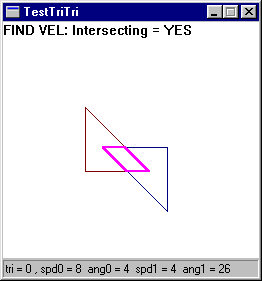
\includegraphics{Figure6.png}

  Figure 6.  Two modified and moved triangles in the \Code{FIND VEL} query,
  both triangles having nonzero velocities, but are intersecting at time $0$.
\end{center}
%
Note that the moved triangles are drawn on top of the original ones, despite
the fact that both have nonzero velocities.  This is the case since $T = 0$
causes the triangles to be moved by a zero distance.

\section{Exiting the Program}

Press the \Code{`q'} or \Code{ESC} keys or select the x--button at the upper
right of the window.

\end{document}
